\newpage
\section{Durchführung}
\label{sec:durchfuerung}

Zur Durchführung des Versuchs werden eine Spektrallampe, optische Elemente, drei Helmholtz-Spulen, eine Dampfzelle mit Heizkörper und ein RF-Generator benötigt.
Die Messdaten werden von einem Lichtdetektor aufgenommen und auf einem Oszilloskop graphisch dargestellt.
Der schematische Aufbau des Versuchs ist in \autoref{fig:aufbau_schem} dargestellt.

\begin{figure}[H]
    \centering
    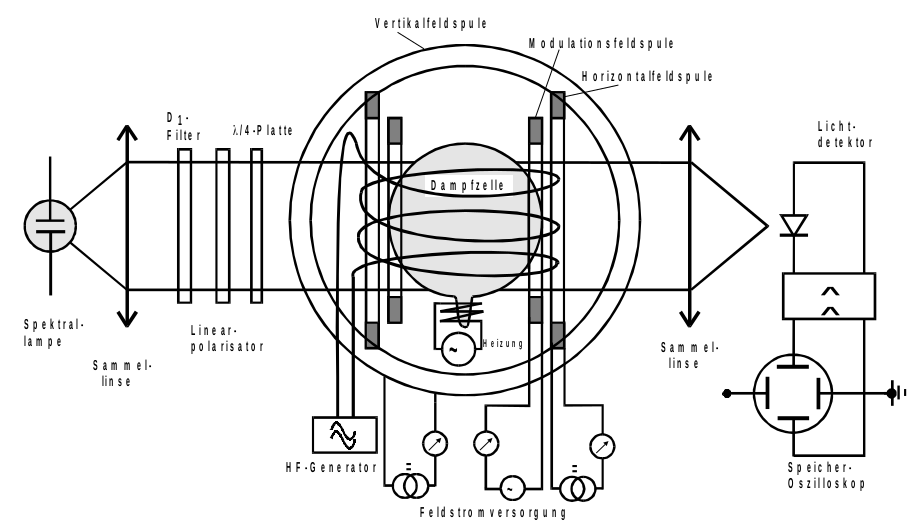
\includegraphics[scale=0.4]{figures/aufbau_schem.png}
    \caption{Dargestellt in dieser Abbildung ist der schematische Aufbau des Versuchs.\cite{V21}}
    \label{fig:aufbau_schem}
\end{figure}

Nachdem die optischen Elemente, das heißt die Sammellinsen, der Wellenlängenfilter, der Polarisationsfilter, sowie die $\lambda/4$-Platte, korrekt eingesetzt und eingestellt wurden, muss der Aufbau lichtundurchlässig bedeckt werden, um Umgebungsrauschen im Detektor zu verhindern.\\
Dies ist in \autoref{fig:aufbau} zu sehen.

\begin{figure}[H]
    \centering
    \subfloat[\centering]{{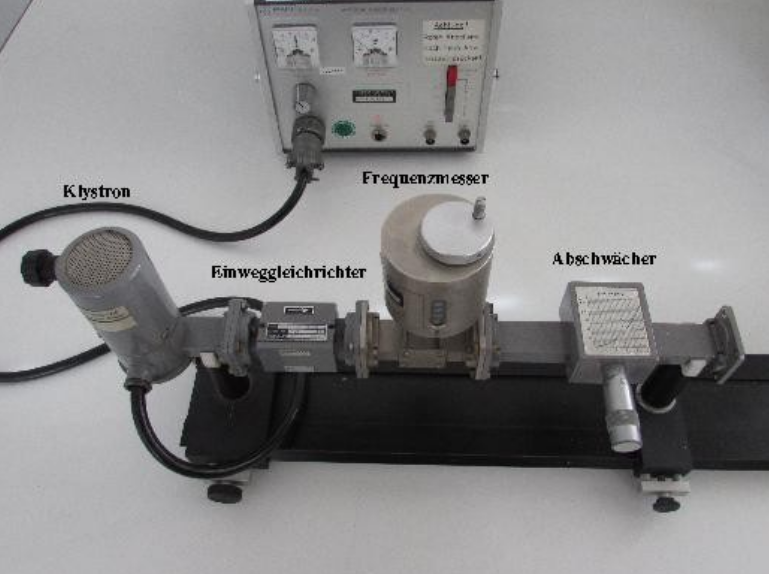
\includegraphics[width=6cm]{figures/aufbau.jpg}}}%
    \qquad
    \subfloat[\centering]{{\includegraphics[width=6cm]{figures/aufbau_verdeckt.jpg}}}%
    \caption{Es ist der Aufbau des Versuches dargestellt, links ohne den Lichtschutz, rechts mit Lichtschutz.}
    \label{fig:aufbau}
\end{figure}

Zu Beginn muss das existierende Erdmagnetfeld kompensiert werden.
Dazu wird die vertikal wirkende Helmholtz-Spule angeschaltet und die Stromzufuhr manuell so geregelt, dass der Detektor ein minimales Signal bei ausgeschaltetem RF-Feld ausgibt.
Das ist der Fall, wenn die Vertikalkomponente des Magnetfeldes kompensiert wurde.\\
Damit der Detektor-output ein weiteres Minimum erreichen kann, soll die Apparatur gedreht werden, bis auch die Horizontalkomponenten des Erdmagnetfelds verschwinden.

\subsection{Landefaktoren und horizontales Erdmagnetfeld}
Zur Bestimmung der Horizontalkomponente des Erdmagnetfelds wird der RF-Generator angeschaltet und eine Frequenz von \SI{100}{\kilo\hertz} bis \SI{1}{\mega\hertz} in \SI{100}{\kilo\hertz}-Schritten angelegt.
Zusätzlich wird mit einem Frequenzgenerator eine \SI{100}{\kilo\hertz}-Sinusspannung an die Steuerapparatur angeschlossen, damit die RF stimulierten Resonanzen auf dem Oszilloskop sichtbar werden.
Da das geheizte Rubidium-Gas aus zwei Isotopen besteht, sind auf dem Bildschirm des Oszilloskops auch zwei korrespondierte Peaks zu sehen.
Dies sind die Resonanzpositionen, an denen das kombinierte Magnetfeld der Sweep-Spule und der horizontalen Helmholtz-Spule ausgelesen wird.
Aus der Steigung der sich so ergebenden Geraden für den gegebenen Frequenzbereich, lassen sich gemäß \autoref{eq:zeeman_frequenz} die Landé-Faktoren berechnen.
\subsection{Kernspin, Isotopenverhältnis und quadratischer Zeeman-Effekt}
Aus den Landé-Faktoren wird der Kernspin der jeweiligen Isotope bestimmt und aus der Höhe der Peaks auf dem Oszilloskop wird das Isotopenverhältnis abgelesen.
Zudem soll der quadratische Zeeman-Effekt für die verwendeten Magnetfelder abgeschätzt werden.
\subsection{Rabi-Oszillationen}
\label{sec:rabi}
Um die Rabi-Oszillationen sichtbar zu machen, wird eine Rechteckspannung mit \SI{5}{\hertz} an die Steuerapparatur angeschlossen.
Nach Justierung des Oszilloskops ist eine exponentiell ansteigende Kurve, gefolgt von gedämpften Oszillationen zu sehen.
Die Amplitude des RF-Generators wird nun in kontinuierlichen Schritten bis \SI{10}{\volt} erhöht und für jede Amplitude die Periode der Rabi-Oszillationen am Oszilloskop abgelesen.
Abschließend wird die Periode gegen die RF-Amplitude graphisch dargestellt und durch eine Hyperbel gefittet.
Das Verhältnis aus den Faktoren des Fits gibt an, wie viel die Messung vom theoretischen Wert abweicht.